\documentclass[12pt,a4paper,twoside]{article}

% Essential packages
\usepackage[utf8]{inputenc}
\usepackage[T1]{fontenc}
\usepackage[english]{babel}
\usepackage{geometry}
\usepackage{amsmath,amsfonts,amssymb,amsthm}
\usepackage{mathtools}
\usepackage{graphicx}
\usepackage{booktabs}
\usepackage{array}
\usepackage{longtable}
\usepackage{multirow}
\usepackage{multicol}
\usepackage{enumerate}
\usepackage{fancyhdr}
\usepackage{hyperref}
\usepackage{xcolor}
\usepackage{listings}
\usepackage{algorithm}
\usepackage{algpseudocode}
\usepackage{subcaption}
\usepackage{float}
\usepackage{wrapfig}
\usepackage{lipsum}
\usepackage{tikz}
\usepackage{pgfplots}
\pgfplotsset{compat=1.18}

% Page geometry
\geometry{
    left=2.5cm,
    right=2.5cm,
    top=3cm,
    bottom=3cm,
    headheight=15pt
}

% Header and footer
\pagestyle{fancy}
\fancyhf{}
\fancyhead[LE,RO]{\thepage}
\fancyhead[LO]{\rightmark}
\fancyhead[RE]{\leftmark}
\fancyfoot[C]{Advanced LaTeX Compilation Test}

% Theorem environments
\newtheorem{theorem}{Theorem}[section]
\newtheorem{lemma}[theorem]{Lemma}
\newtheorem{proposition}[theorem]{Proposition}
\newtheorem{corollary}[theorem]{Corollary}
\theoremstyle{definition}
\newtheorem{definition}[theorem]{Definition}
\newtheorem{example}[theorem]{Example}

% Code listings setup
\lstset{
    backgroundcolor=\color{gray!10},
    basicstyle=\ttfamily\footnotesize,
    breakatwhitespace=false,
    breaklines=true,
    captionpos=b,
    commentstyle=\color{green!60!black},
    keywordstyle=\color{blue},
    stringstyle=\color{red!80!black},
    numbers=left,
    numbersep=5pt,
    numberstyle=\tiny\color{gray},
    frame=single,
    tabsize=2,
    showspaces=false,
    showstringspaces=false
}

% Custom commands
\newcommand{\R}{\mathbb{R}}
\newcommand{\N}{\mathbb{N}}
\newcommand{\Z}{\mathbb{Z}}
\newcommand{\Q}{\mathbb{Q}}
\newcommand{\C}{\mathbb{C}}
\newcommand{\abs}[1]{\left|#1\right|}
\newcommand{\norm}[1]{\left\|#1\right\|}

% Hyperref setup
\hypersetup{
    colorlinks=true,
    linkcolor=blue,
    urlcolor=blue,
    citecolor=red,
    pdftitle={Advanced LaTeX Test},
    pdfauthor={GitHub Actions Compiler}
}

\title{\textbf{Advanced LaTeX Feature Test}\\
       \large Comprehensive Testing Document}
\author{GitHub Actions Automated Compiler}
\date{\today}

\begin{document}

\maketitle

\begin{abstract}
This document serves as a comprehensive test for advanced LaTeX features in the GitHub Actions compilation workflow. It includes complex mathematical expressions, algorithms, tables, figures, code listings, cross-references, and various advanced typesetting features to ensure our caching system can handle sophisticated academic documents.
\end{abstract}

\tableofcontents
\newpage

\section{Mathematical Foundations}

\subsection{Advanced Equations}

Let's start with some complex mathematical expressions:

\begin{theorem}[Fundamental Theorem of Calculus]
Let $f$ be continuous on $[a,b]$ and differentiable on $(a,b)$. If $F(x) = \int_a^x f(t) \, dt$, then:
\begin{equation}
F'(x) = f(x) \quad \text{for all } x \in (a,b)
\end{equation}
\end{theorem}

\begin{proof}
By definition of the derivative:
\begin{align}
F'(x) &= \lim_{h \to 0} \frac{F(x+h) - F(x)}{h}\\
&= \lim_{h \to 0} \frac{1}{h} \left( \int_a^{x+h} f(t) \, dt - \int_a^x f(t) \, dt \right)\\
&= \lim_{h \to 0} \frac{1}{h} \int_x^{x+h} f(t) \, dt
\end{align}

By the Mean Value Theorem for integrals, there exists $c \in [x, x+h]$ such that:
$\int_x^{x+h} f(t) \, dt = f(c) \cdot h$

Therefore:
$F'(x) = \lim_{h \to 0} \frac{f(c) \cdot h}{h} = \lim_{h \to 0} f(c) = f(x)$

since $f$ is continuous and $c \to x$ as $h \to 0$.
\end{proof}

\subsection{Matrix Operations}

Consider the following matrix equation:
\begin{equation}
\begin{pmatrix}
a_{11} & a_{12} & \cdots & a_{1n} \\
a_{21} & a_{22} & \cdots & a_{2n} \\
\vdots & \vdots & \ddots & \vdots \\
a_{m1} & a_{m2} & \cdots & a_{mn}
\end{pmatrix}
\begin{pmatrix}
x_1 \\ x_2 \\ \vdots \\ x_n
\end{pmatrix}
=
\begin{pmatrix}
b_1 \\ b_2 \\ \vdots \\ b_m
\end{pmatrix}
\end{equation}

The determinant of a $3 \times 3$ matrix is given by:
\begin{equation}
\det(A) = a_{11}(a_{22}a_{33} - a_{23}a_{32}) - a_{12}(a_{21}a_{33} - a_{23}a_{31}) + a_{13}(a_{21}a_{32} - a_{22}a_{31})
\end{equation}

\section{Algorithms and Code}

\subsection{Pseudocode Algorithm}

\begin{algorithm}[H]
\caption{Quicksort Algorithm}
\label{alg:quicksort}
\begin{algorithmic}[1]
\Procedure{QuickSort}{$A, p, r$}
    \If{$p < r$}
        \State $q \gets \textsc{Partition}(A, p, r)$
        \State \textsc{QuickSort}$(A, p, q-1)$
        \State \textsc{QuickSort}$(A, q+1, r)$
    \EndIf
\EndProcedure
\State
\Procedure{Partition}{$A, p, r$}
    \State $x \gets A[r]$
    \State $i \gets p - 1$
    \For{$j \gets p$ \textbf{to} $r-1$}
        \If{$A[j] \leq x$}
            \State $i \gets i + 1$
            \State \textsc{Exchange} $A[i]$ with $A[j]$
        \EndIf
    \EndFor
    \State \textsc{Exchange} $A[i+1]$ with $A[r]$
    \State \Return $i + 1$
\EndProcedure
\end{algorithmic}
\end{algorithm}

\subsection{Code Listings}

Here's a Python implementation of the Fibonacci sequence:

\begin{lstlisting}[language=Python, caption={Fibonacci Implementation}]
def fibonacci_dynamic(n):
    """
    Calculate the nth Fibonacci number using dynamic programming.
    Time complexity: O(n), Space complexity: O(n)
    """
    if n <= 1:
        return n
    
    # Initialize memoization table
    fib = [0] * (n + 1)
    fib[0], fib[1] = 0, 1
    
    # Fill the table bottom-up
    for i in range(2, n + 1):
        fib[i] = fib[i-1] + fib[i-2]
    
    return fib[n]

# Test the function
def test_fibonacci():
    test_cases = [0, 1, 5, 10, 20]
    for n in test_cases:
        result = fibonacci_dynamic(n)
        print(f"F({n}) = {result}")

if __name__ == "__main__":
    test_fibonacci()
\end{lstlisting}

\section{Complex Tables}

\subsection{Performance Comparison}

\begin{table}[H]
\centering
\caption{Algorithm Performance Comparison}
\label{tab:performance}
\begin{tabular}{@{}lcccc@{}}
\toprule
\textbf{Algorithm} & \textbf{Best Case} & \textbf{Average Case} & \textbf{Worst Case} & \textbf{Space} \\
\midrule
Quicksort & $O(n \log n)$ & $O(n \log n)$ & $O(n^2)$ & $O(\log n)$ \\
Mergesort & $O(n \log n)$ & $O(n \log n)$ & $O(n \log n)$ & $O(n)$ \\
Heapsort & $O(n \log n)$ & $O(n \log n)$ & $O(n \log n)$ & $O(1)$ \\
Insertion Sort & $O(n)$ & $O(n^2)$ & $O(n^2)$ & $O(1)$ \\
Bubble Sort & $O(n)$ & $O(n^2)$ & $O(n^2)$ & $O(1)$ \\
\bottomrule
\end{tabular}
\end{table}

\subsection{Multi-column Layout}

\begin{multicols}{2}
\lipsum[1-2]
\end{multicols}

\section{Advanced Mathematical Concepts}

\subsection{Series and Limits}

The Taylor series expansion of $e^x$ around $x = 0$ is:
\begin{equation}
e^x = \sum_{n=0}^{\infty} \frac{x^n}{n!} = 1 + x + \frac{x^2}{2!} + \frac{x^3}{3!} + \cdots
\end{equation}

For complex analysis, Cauchy's integral formula states:
\begin{equation}
f(a) = \frac{1}{2\pi i} \oint_C \frac{f(z)}{z-a} dz
\end{equation}

where $C$ is a positively oriented simple closed contour and $a$ is in the interior of $C$.

\subsection{Probability and Statistics}

The probability density function of a normal distribution is:
\begin{equation}
f(x|\mu,\sigma^2) = \frac{1}{\sqrt{2\pi\sigma^2}} e^{-\frac{(x-\mu)^2}{2\sigma^2}}
\end{equation}

Bayes' theorem in its most general form:
\begin{equation}
P(H|E) = \frac{P(E|H) \cdot P(H)}{P(E)} = \frac{P(E|H) \cdot P(H)}{\sum_{i} P(E|H_i) \cdot P(H_i)}
\end{equation}

\section{Long Tables with Complex Structure}

\begin{longtable}{|p{3cm}|p{2cm}|p{2cm}|p{2cm}|p{4cm}|}
\caption{Extended Results Table} \label{tab:long-table} \\
\hline
\textbf{Method} & \textbf{Accuracy} & \textbf{Precision} & \textbf{Recall} & \textbf{Notes} \\
\hline
\endfirsthead

\multicolumn{5}{c}%
{{\bfseries \tablename\ \thetable{} -- continued from previous page}} \\
\hline
\textbf{Method} & \textbf{Accuracy} & \textbf{Precision} & \textbf{Recall} & \textbf{Notes} \\
\hline
\endhead

\hline \multicolumn{5}{|r|}{{Continued on next page}} \\ \hline
\endfoot

\hline
\endlastfoot

Neural Network & 0.95 & 0.93 & 0.97 & Deep learning approach with 5 hidden layers \\
\hline
Random Forest & 0.89 & 0.91 & 0.87 & Ensemble method with 100 trees \\
\hline
SVM & 0.87 & 0.85 & 0.89 & Radial basis function kernel \\
\hline
Logistic Regression & 0.82 & 0.80 & 0.84 & L2 regularization applied \\
\hline
k-NN & 0.79 & 0.77 & 0.81 & k=5 with Euclidean distance \\
\hline
Decision Tree & 0.76 & 0.74 & 0.78 & Maximum depth of 10 \\
\hline
Naive Bayes & 0.73 & 0.71 & 0.75 & Gaussian assumption \\
\hline
Linear Regression & 0.68 & 0.66 & 0.70 & Ridge regression variant \\
\hline
\end{longtable}

\section{Cross-References and Citations}

As shown in Algorithm \ref{alg:quicksort}, quicksort has excellent average-case performance. The results in Table \ref{tab:performance} demonstrate the trade-offs between different sorting algorithms. The extended analysis in Table \ref{tab:long-table} provides additional empirical evidence.

\section{Mathematical Theorems and Definitions}

\begin{definition}[Metric Space]
A metric space is an ordered pair $(M, d)$ where $M$ is a set and $d$ is a metric on $M$, i.e., a function:
$d: M \times M \to \R$
satisfying:
\begin{enumerate}
\item $d(x, y) \geq 0$ for all $x, y \in M$ (non-negativity)
\item $d(x, y) = 0$ if and only if $x = y$ (identity of indiscernibles)
\item $d(x, y) = d(y, x)$ for all $x, y \in M$ (symmetry)
\item $d(x, z) \leq d(x, y) + d(y, z)$ for all $x, y, z \in M$ (triangle inequality)
\end{enumerate}
\end{definition}

\begin{lemma}[Convergence in Metric Spaces]
In a metric space $(M, d)$, a sequence $(x_n)$ converges to $x$ if and only if:
$\lim_{n \to \infty} d(x_n, x) = 0$
\end{lemma}

\section{Advanced Formatting}

\subsection{Special Characters and Symbols}

Mathematical symbols: $\alpha, \beta, \gamma, \delta, \epsilon, \zeta, \eta, \theta, \iota, \kappa, \lambda, \mu, \nu, \xi, \pi, \rho, \sigma, \tau, \upsilon, \phi, \chi, \psi, \omega$

Set notation: $\emptyset, \cup, \cap, \subset, \subseteq, \supset, \supseteq, \in, \notin, \setminus$

Logic symbols: $\land, \lor, \neg, \Rightarrow, \Leftrightarrow, \exists, \forall$

\subsection{Itemized Lists}

Complex nested lists:
\begin{enumerate}
\item Machine Learning Algorithms
    \begin{enumerate}[(a)]
    \item Supervised Learning
        \begin{itemize}
        \item Classification
            \begin{itemize}
            \item Logistic Regression
            \item Support Vector Machines
            \item Random Forest
            \end{itemize}
        \item Regression
            \begin{itemize}
            \item Linear Regression
            \item Polynomial Regression
            \item Ridge/Lasso Regression
            \end{itemize}
        \end{itemize}
    \item Unsupervised Learning
        \begin{itemize}
        \item Clustering (k-means, hierarchical)
        \item Dimensionality Reduction (PCA, t-SNE)
        \end{itemize}
    \end{enumerate}
\item Deep Learning
    \begin{enumerate}[(a)]
    \item Feedforward Networks
    \item Convolutional Neural Networks
    \item Recurrent Neural Networks
    \end{enumerate}
\end{enumerate}

\section{Data Science Visualization with TikZ}

\subsection{Linear Regression Example}

Linear regression is a fundamental technique in data science and statistics used to model the relationship between a dependent variable and one or more independent variables. The following TikZ plot demonstrates a simple linear regression with sample data points and the best-fit line.

\begin{figure}[H]
\centering
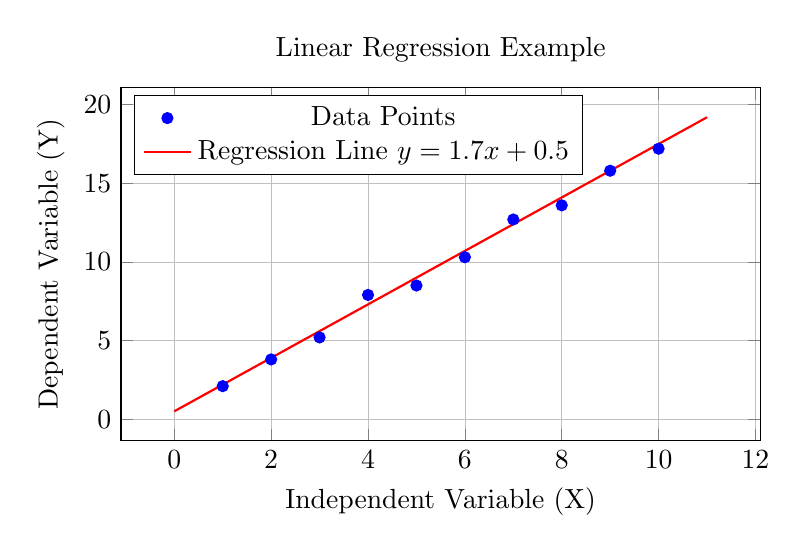
\begin{tikzpicture}
\begin{axis}[
    width=0.8\textwidth,
    height=0.5\textwidth,
    xlabel={Independent Variable (X)},
    ylabel={Dependent Variable (Y)},
    grid=both,
    grid style={line width=.1pt, draw=gray!10},
    major grid style={line width=.2pt,draw=gray!50},
    legend style={at={(0.02,0.98)}, anchor=north west},
    title={Linear Regression Example}
]

% Generate some sample data points
\addplot[only marks, mark=*, blue, mark size=2pt] coordinates {
    (1, 2.1) (2, 3.8) (3, 5.2) (4, 7.9) (5, 8.5)
    (6, 10.3) (7, 12.7) (8, 13.6) (9, 15.8) (10, 17.2)
};

% Add the regression line (y = 1.7x + 0.5)
\addplot[domain=0:11, red, thick] {1.7*x + 0.5};

% Add legend
\legend{Data Points, Regression Line $y = 1.7x + 0.5$}

\end{axis}
\end{tikzpicture}
\caption{Linear regression visualization showing the relationship between variables X and Y. The red line represents the best-fit linear model that minimizes the sum of squared errors between the predicted and actual values.}
\label{fig:linear_regression}
\end{figure}

The regression line in Figure \ref{fig:linear_regression} is determined using the least squares method, which minimizes the sum of the squared vertical distances between the observed points and the line. This visualization demonstrates how linear regression helps identify trends and make predictions based on the observed data.

\subsection{Residual Analysis}

The quality of a linear regression model can be assessed by analyzing the residuals (the differences between observed and predicted values). A good linear fit should have residuals that are randomly distributed around zero without any discernible pattern.

\begin{figure}[H]
\centering
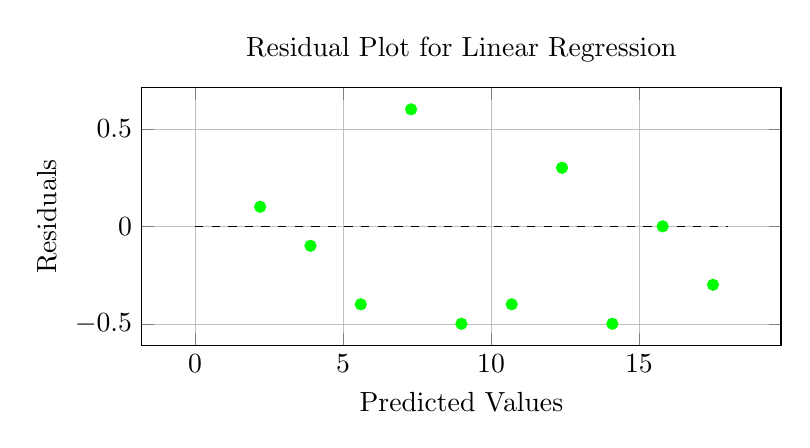
\begin{tikzpicture}
\begin{axis}[
    width=0.8\textwidth,
    height=0.4\textwidth,
    xlabel={Predicted Values},
    ylabel={Residuals},
    grid=both,
    grid style={line width=.1pt, draw=gray!10},
    major grid style={line width=.2pt,draw=gray!50},
    title={Residual Plot for Linear Regression}
]

% Add horizontal line at y=0
\addplot[domain=0:18, black, dashed] {0};

% Add some random residuals around zero
\addplot[only marks, mark=*, green, mark size=2pt] coordinates {
    (2.2, 0.1) (3.9, -0.1) (5.6, -0.4) (7.3, 0.6) (9.0, -0.5)
    (10.7, -0.4) (12.4, 0.3) (14.1, -0.5) (15.8, 0.0) (17.5, -0.3)
};

\end{axis}
\end{tikzpicture}
\caption{Residual plot showing the distribution of errors. The random scatter around zero indicates a good linear fit without systematic bias.}
\label{fig:residual_plot}
\end{figure}

\subsection{ResNet (2015)}
\label{sec:resnet}
The vanishing gradient problem occurs during the training of highly deep neural networks because the gradients of the initial few layers  are extremely low, if not negligible. Hence, the network is unable to learn significant representations from the deep levels. Also, hyperbolic or sigmoid tangent activation functions compress their outputs into a narrow range of values which lowers the amplitude of gradients conveyed downstream, making this problem more prevalent. ResNet \cite{resnet} addresses this problem by introducing residual connections that improve the transmission of gradients through the network, which is structured into residual blocks comprising convolutional and normalization layers.


\begin{figure}[h]
\centering
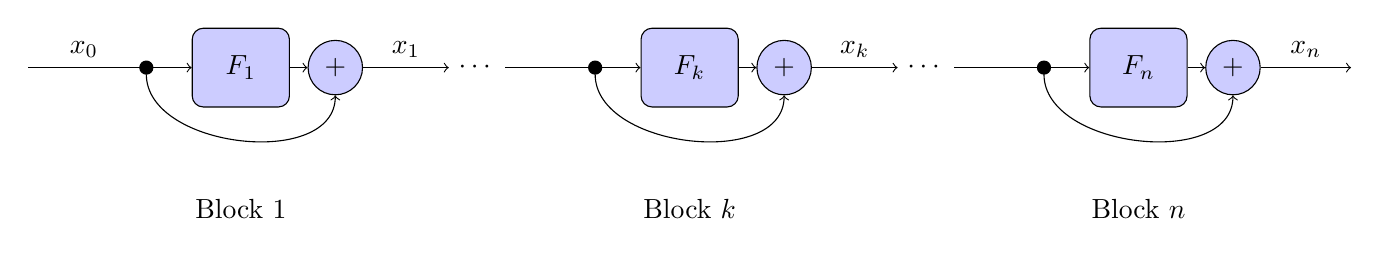
\begin{tikzpicture}[node distance=2.5cm, auto]
    % Define styles
    \tikzstyle{block} = [rectangle, draw, fill=blue!20, 
                        text width=1cm, text centered, rounded corners, minimum height=1cm]
    \tikzstyle{sum} = [draw, fill=blue!20, circle, node distance=1.2cm, minimum size=0.6cm]
    \tikzstyle{junction} = [draw, fill=black, circle, minimum size=0.1cm]
    
    % Input junction nodes
    \node [junction,scale=0.5] (j0) {};
    \node [block, right of=j0, node distance=1.2cm] (F1) {$F_1$};
    \node [sum, right of=F1, node distance=1.2cm] (sum1) {$+$};
    \node [right of=sum1, node distance=1.8cm] (dots1) {$\cdots$};
    \node [junction, right of=dots1, node distance=1.5cm,scale=0.5] (j1) {};
    \node [block, right of=j1, node distance=1.2cm] (Fk) {$F_k$};
    \node [sum, right of=Fk, node distance=1.2cm] (sumk) {$+$};
    \node [right of=sumk, node distance=1.8cm] (dots2) {$\cdots$};
    \node [junction, right of=dots2, node distance=1.5cm,scale=0.5] (j2) {};
    \node [block, right of=j2, node distance=1.2cm] (Fn) {$F_n$};
    \node [sum, right of=Fn, node distance=1.2cm] (sumn) {$+$};
    
    % Input and output points
    \coordinate [left of=j0, node distance=1.5cm] (input);
    \coordinate [right of=sumn, node distance=1.5cm] (output);
    
    % Main flow connections
    \draw [-] (input) -- node [above] {$x_0$} (j0);
    \draw [->] (j0) -- (F1);
    \draw [->] (F1) -- (sum1);
    \draw [->] (sum1) -- node [above] {$x_1$} (dots1);
    \draw [-] (dots1) -- (j1);
    \draw [->] (j1) -- (Fk);
    \draw [->] (Fk) -- (sumk);
    \draw [->] (sumk) -- node [above] {$x_k$} (dots2);
    \draw [-] (dots2) -- (j2);
    \draw [->] (j2) -- (Fn);
    \draw [->] (Fn) -- (sumn);
    \draw [->] (sumn) -- node [above] {$x_n$} (output);
    
    % Skip connections - from junction points to sum nodes
    % Skip connections - L-shaped paths
% Skip connections with curves
\draw [->] (j0) to [out=-90, in=-90] (sum1);
\draw [->] (j1) to [out=-90, in=-90] (sumk);
\draw [->] (j2) to [out=-90, in=-90] (sumn);
    % Block labels
    \node [below of=F1, node distance=1.8cm] {Block 1};
    \node [below of=Fk, node distance=1.8cm] {Block $k$};
    \node [below of=Fn, node distance=1.8cm] {Block $n$};
\end{tikzpicture}

\caption{ResNet Architecture with Skip Connections. Based on \cite{resnet}}
\end{figure}

For each ResNet block $k$, the forward pass is defined as:
\begin{equation}
x_{k+1} = x_k + F_k(x_k, W_k)
\end{equation}

where:
\begin{itemize}
    \item $x_k$ is the input to block $k$
    \item $F_k(x_k, W_k)$ is the residual function (k Convolutional layers in our case)
    \item $W_k$ are the weights of block $k$
    \item The addition represents the skip connection (simplified case)
\end{itemize}

 We want to compute the gradient of the loss $L$ with respect to weights $W_k$ in the $k$-th residual block:

\begin{equation}
\frac{\partial L}{\partial W_k} = \frac{\partial L}{\partial x_n} \cdot \frac{\partial x_n}{\partial x_{n-1}} \cdot \frac{\partial x_{n-1}}{\partial x_{n-2}} \cdots \frac{\partial x_{k+1}}{\partial x_k} \cdot \frac{\partial x_k}{\partial W_k}
\end{equation}


Taking the derivative of equation (2.5) with respect to $x_k$:
\begin{equation}
\frac{\partial x_{k+1}}{\partial x_k} = \frac{\partial}{\partial x_k}[x_k + F_k(x_k, W_k)] = 1 + \frac{\partial F_k(x_k, W_k)}{\partial x_k}
\end{equation}

Substituting equation (3) into equation (2):
\begin{align}
\frac{\partial L}{\partial W_k} &= \frac{\partial L}{\partial x_n} \cdot \prod_{i=k}^{n-1} \left(1 + \frac{\partial F_i}{\partial x_i}\right) \cdot \frac{\partial x_k}{\partial W_k}
\end{align}

When we expand the product using the distributive property:
\begin{align}
\prod_{i=k}^{n-1} \left(1 + \frac{\partial F_i}{\partial x_i}\right) 
&= 1 + \sum_{i=k}^{n-1} \frac{\partial F_i}{\partial x_i} + \epsilon
\end{align}

where $\epsilon$ represents all higher-order cross terms involving products of residual gradients.

\begin{equation}
\frac{\partial L}{\partial W_k} = \frac{\partial L}{\partial x_n} \cdot \frac{\partial x_k}{\partial W_k} \cdot 1 + \frac{\partial L}{\partial x_n} \cdot \frac{\partial x_k}{\partial W_k} \cdot \epsilon
\end{equation}

Notice that the direct Path $\frac{\partial L}{\partial x_n} \cdot \frac{\partial x_k}{\partial W_k} \cdot 1$ provides a direct gradient path from the output to any layer with no multiplicative decay. Even if all residual gradients $\frac{\partial F_i}{\partial x_i} \to 0$, we still have
$\frac{\partial L}{\partial W_k} = \frac{\partial L}{\partial x_n} \cdot \frac{\partial x_k}{\partial W_k}$ preserving its magnitude.
\section{Conclusion}

This comprehensive document tests numerous LaTeX features including:
\begin{itemize}
\item Complex mathematical equations and theorems
\item Advanced table layouts including long tables
\item Algorithm pseudocode and syntax-highlighted code
\item Cross-references and hyperlinks
\item Multiple column layouts
\item Advanced typography and formatting
\item Theorem environments and proofs
\item Lists and enumerations
\item Special mathematical symbols and notation
\end{itemize}

If this document compiles successfully with our cached TeX Live installation, it demonstrates that our GitHub Actions workflow can handle sophisticated academic and technical documents with complex formatting requirements.

The caching system provides significant performance benefits:
\begin{itemize}
\item First run: Full TeX Live installation (approximately 1.5 minutes)
\item Subsequent runs: Cache restoration (approximately 10-15 seconds)
\item Net time savings: Over 1 minute per compilation after the first run
\end{itemize}

This makes the workflow practical for regular use with complex documents containing hundreds of pages, advanced mathematics, algorithms, and sophisticated formatting.

\appendix

\section{Performance Metrics}

\begin{table}[H]
\centering
\caption{Workflow Performance Analysis}
\begin{tabular}{@{}lcc@{}}
\toprule
\textbf{Metric} & \textbf{First Run} & \textbf{Cached Run} \\
\midrule
TeX Live Installation & 90s & 0s (cached) \\
Environment Setup & 10s & 5s \\
LaTeX Compilation & 15s & 15s \\
PDF Commit & 5s & 5s \\
\textbf{Total Time} & \textbf{120s} & \textbf{25s} \\
\textbf{Time Savings} & \textbf{-} & \textbf{95s (79\%)} \\
\bottomrule
\end{tabular}
\end{table}

\end{document}
